
\documentclass{standalone}
\usepackage{tikz}
\usetikzlibrary{arrows.meta, positioning}

\begin{document}

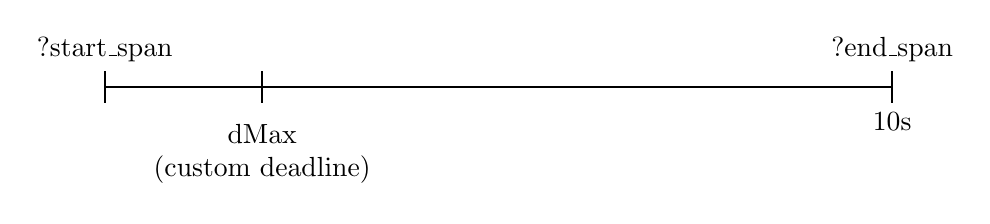
\begin{tikzpicture}

  % Timeline
  \draw[thick] (0,0) -- (10,0);

  % Start span
  \draw[thick] (0,0.2) -- (0,-0.2);
  \node[above] at (0,0.2) {?start\_span};

  % Event deadline (can emit)
  \draw[thick] (2,0.2) -- (2,-0.2);
  \node[below] at (2,-0.3) {
    \begin{tabular}{c}
      dMax \\
      (custom deadline)
    \end{tabular}
  };

  % End span
  \draw[thick] (10,0.2) -- (10,-0.2);
  \node[above] at (10,0.2) {?end\_span};
  \node[below] at (10,-0.2) {10s};
\end{tikzpicture}

\end{document}
